
\section{Design methodology: from requirements to final design}

We follow an iterative engineering process: specifying numbered requirements (Section 4.1), comparing alternatives against weighted criteria (Section 4.2), then prototyping, measuring and refining. The model follows its own inner loop of collecting clips, training, evaluating on the validation split, recording hard negatives that target the errors, and retraining. Only once a model meets the targets on the Pi do we freeze it and run the test set, a single time (Figure \ref{fig:ch5-01}).

\begin{figure}[htbp]
  \centering
  \resizebox{\linewidth}{!}{\begin{tikzpicture}[node distance=6mm and 8mm]
  % design
  \fcard{s1}{sbgray}{\faListUl}{Specify requirements}{}
  \fcard{s2}{sbgray}{\faSearch}{Survey alternatives}{right=of s1}
  \fcard{s3}{sbgray}{\faBalanceScale}{Score and select}{right=of s2}
  \fcard{s4}{sbgray}{\faTools}{Build prototype}{right=of s3}
  % model loop
  \fcard{m1}{sbblue}{\faVideo}{Collect clips}{below=16mm of s1}
  \fcard{m2}{sbblue}{\faCogs}{Train or fine-tune}{right=of m1}
  \fcard{m3}{sbblue}{\faChartBar}{Evaluate on validation}{right=of m2}
  \fcard{m4}{sbblue}{\faSearchPlus}{Error analysis}{below=of m3}
  \fcard{m5}{sbblue}{\faTimesCircle}{Record hard negatives}{below=of m2}
  % verify
  \fcard{v1}{sbgreen}{\faMicrochip}{Measure on the Pi 5}{right=18mm of m3}
  \fdec{v2}{sbgreen}{Meets the spec?}{below=of v1}
  \fterm{v3}{sbgreen}{Freeze, test once}{below=of v2}
  \draw[farr] (s1) -- (s2); \draw[farr] (s2) -- (s3); \draw[farr] (s3) -- (s4);
  \draw[farr] (s4.south) -- ++(0,-5mm) -| (m1.north);
  \draw[farr] (m1) -- (m2); \draw[farr] (m2) -- (m3); \draw[farr] (m3) -- (m4);
  \draw[farr] (m4) -- (m5); \draw[farr] (m5) -- (m2);
  \draw[farr] (m3) -- (v1); \draw[farr] (v1) -- (v2);
  \draw[farr] (v2) -- node[flab, right]{yes} (v3);
  \draw[farr] (v2.west) -- node[flab, above]{no} (m4.east);
  \begin{scope}[on background layer]
    \node[freg=sbgray, fit=(s1)(s4), label={[freglab]north west:Design}] {};
    \node[freg=sbblue, fit=(m1)(m3)(m5)(m4), label={[freglab]north west:Model loop}] {};
    \node[freg=sbgreen, fit=(v1)(v3), label={[freglab]north west:Verify}] {};
  \end{scope}
\end{tikzpicture}
}
  \caption{Design process with the repeating model loop}
  \label{fig:ch5-01}
\end{figure}

\section{Skills, techniques, models and tools needed}

Table \ref{tab:ch5-tools} lists the skills and tools the project requires, all of which are free or open source.

\begin{table}[htbp]
\centering
\caption{Skills, tools and licences}
\label{tab:ch5-tools}
\footnotesize
\setlength{\tabcolsep}{3pt}
\renewcommand{\arraystretch}{1.15}
\begin{tabular}{|p{0.150\linewidth}|p{0.470\linewidth}|p{0.310\linewidth}|}
\hline
\textbf{Area} & \textbf{Skills and tools} & \textbf{Licence or cost} \\
\hline
Model & Python, PyTorch, Ultralytics \gls{yolo}11, transfer learning, structured pruning, \gls{ptq} and \gls{qat}, TensorBoard & AGPL-3.0 for Ultralytics, which needs open-sourcing or an enterprise licence if the product is sold \\
\hline
Data & CVAT annotation, OpenCV, the subject-disjoint protocol & Free \\
\hline
Embedded & Raspberry Pi OS, Hailo runtime and Dataflow Compiler, \gls{gpio}, boot services, one small C++ library & Free with a Hailo developer account \\
\hline
Server and web & SQLite, FastAPI, PostgreSQL, React, free hosting tiers, OpenStreetMap Overpass \gls{api} \cite{r68} & Free, maps under ODbL with attribution \\
\hline
Design & Git and GitHub, draw.io, Mermaid, TikZ, Blender, \gls{matlab} for the alert sounds & Free or university licence \\
\hline
Measurement & Multimeter, inline \gls{usb}-C power meter, infrared thermometer, phone filming at 240 \gls{fps} & Lab stock \\
\hline
\end{tabular}
\end{table}


\section{Dataset: Collection, Labelling, Splits and Hard Negatives}
\label{sec:dataset}
\subsection{Dataset goals and overview}

The dataset must teach the detector our four classes from our own camera view, while allowing us to measure how well the model generalises to people it has never seen. Besides the four positive classes, every frame without a cue serves as a negative, with hard negatives added in a second round. Table \ref{tab:ch5-01} gives the plan.

\begin{table}[htbp]
\centering
\caption{Planned dataset}
\label{tab:ch5-01}
\footnotesize
\setlength{\tabcolsep}{3pt}
\renewcommand{\arraystretch}{1.15}
\begin{tabular}{|p{0.300\linewidth}|p{0.630\linewidth}|}
\hline
\textbf{Item} & \textbf{Plan} \\
\hline
Subjects & The four authors (S01 to S04), with appearance variety coming from pre-training on the 14 drivers of DMD \\
\hline
Sessions & Several 10-minute sessions per subject, in the afternoon and in the evening, each with a 20\,s neutral baseline \\
\hline
Hours of video & About 2.7 hours (at least four sessions per subject), plus about 0.5 hours of hard-negative clips \\
\hline
Frame counts & Labelled at 5 \gls{fps}: about 48{,}000 frames, of which roughly 15--20\% contain a cue \\
\hline
Classes & Yawning, hand-over-mouth, drinking, phone use, plus negatives (including looking away) \\
\hline
\end{tabular}
\end{table}

\subsection{Collection protocol}
\subsubsection{Recording setup and conditions}

The camera is mounted in the target in-car position (Figure \ref{fig:ch4-09}). Each subject sits in a parked car with the engine off and records several 10-minute \gls{rgb} sessions at 1080p and 30 \gls{fps}, in the afternoon and in the evening. Following the guideline in Figure \ref{fig:ch5-guide}, the subject performs each behaviour several times at random moments, separated by periods of normal posture. Looking away is recorded deliberately and labelled as a negative, so that mirror checks teach the model what not to alert on.

\begin{figure}[htbp]
\centering
\begin{subfigure}[t]{0.31\linewidth}\centering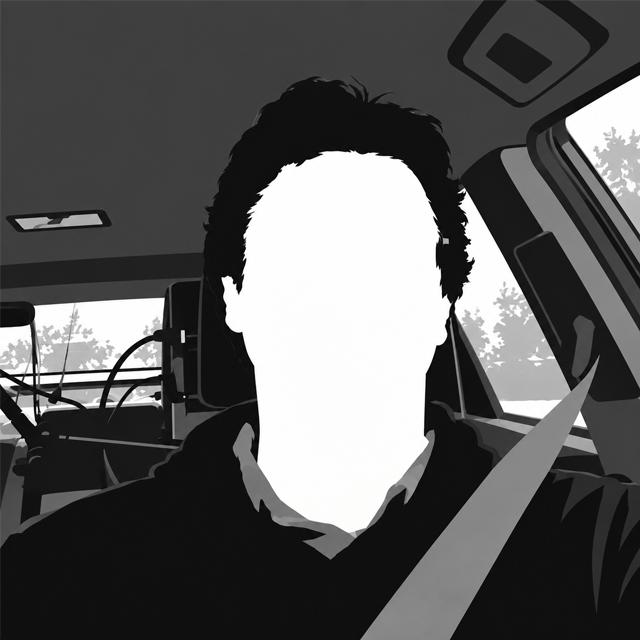
\includegraphics[width=\linewidth]{Figures/guide_0.png}\caption{Seating position}\end{subfigure}\hfill
\begin{subfigure}[t]{0.31\linewidth}\centering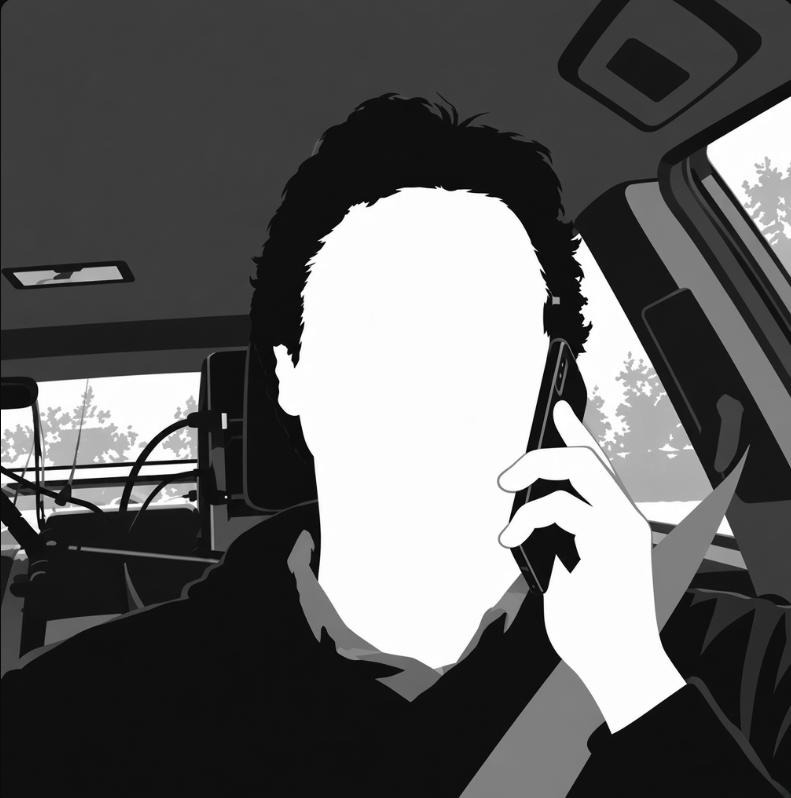
\includegraphics[width=\linewidth]{Figures/guide_1.png}\caption{Holding a phone}\end{subfigure}\hfill
\begin{subfigure}[t]{0.31\linewidth}\centering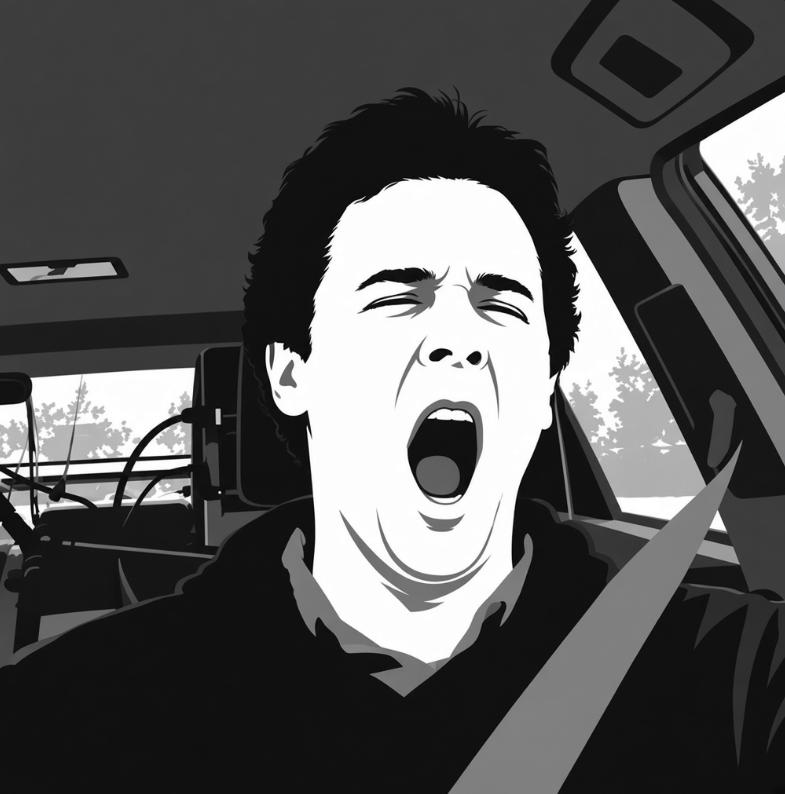
\includegraphics[width=\linewidth]{Figures/guide_2.png}\caption{Yawning}\end{subfigure}\\[2mm]
\begin{subfigure}[t]{0.31\linewidth}\centering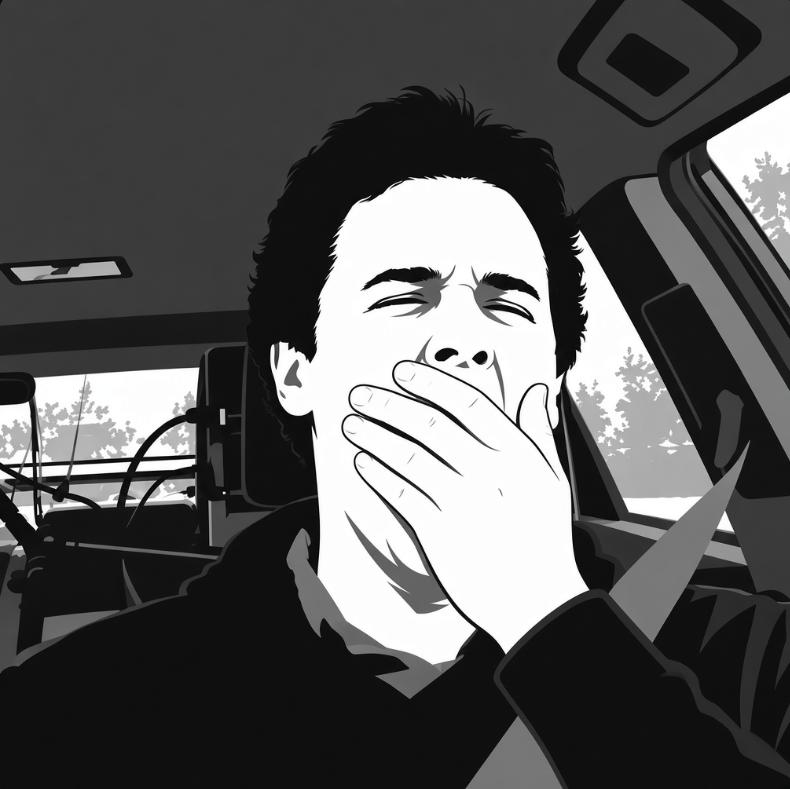
\includegraphics[width=\linewidth]{Figures/guide_3.png}\caption{Covering a yawn}\end{subfigure}\hfill
\begin{subfigure}[t]{0.31\linewidth}\centering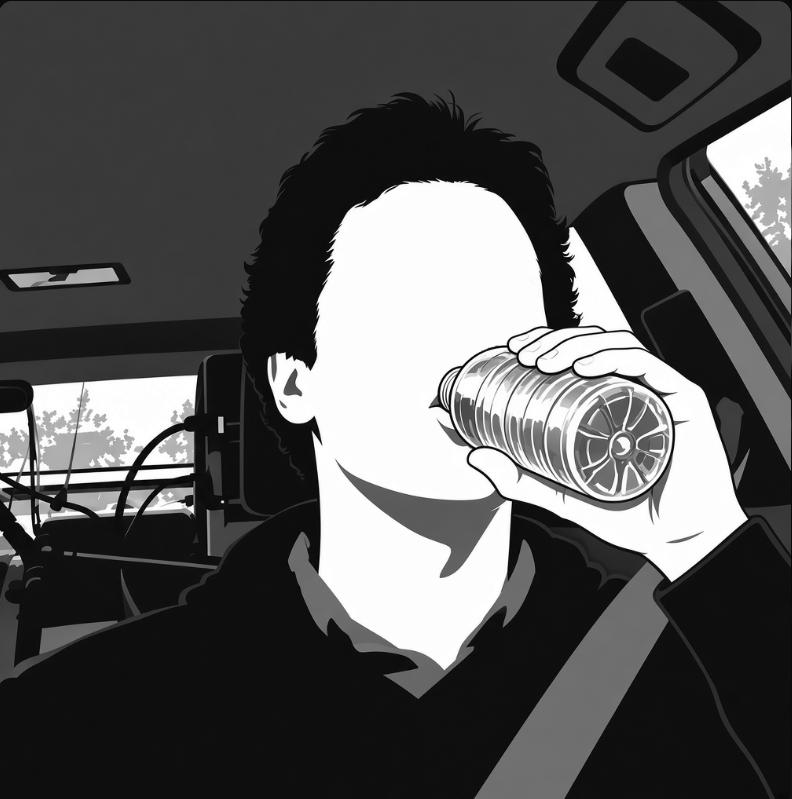
\includegraphics[width=\linewidth]{Figures/guide_4.png}\caption{Drinking}\end{subfigure}\hfill
\begin{subfigure}[t]{0.31\linewidth}\centering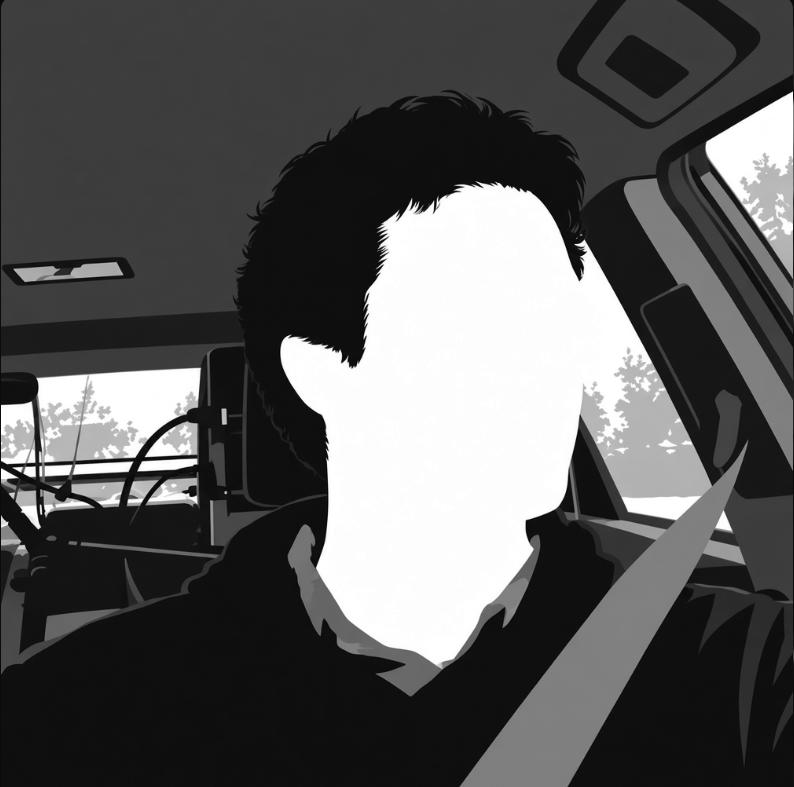
\includegraphics[width=\linewidth]{Figures/guide_5.png}\caption{Looking away (negative)}\end{subfigure}
\caption{Recording guideline given to every subject}
\label{fig:ch5-guide}
\end{figure}

\subsubsection{Pilot sessions and what they taught us}
\label{sec:pilot}

Before the C922 arrived, three of the authors (P1 to P3) recorded four pilot sessions in three cars, by day and by night, using phones in different mounts (Table \ref{tab:ch5-pilot} and Figure \ref{fig:ch5-pilot}). These clips are neither labelled nor part of the dataset, as we used them only to check the protocol and the camera mount by eye. Two of them were filmed upside down, showing that the frame grabber needs a 180$^\circ$ rotation setting.

\begin{table}[htbp]
\centering
\caption{Pilot sessions recorded in November 2026}
\label{tab:ch5-pilot}
\footnotesize
\setlength{\tabcolsep}{3pt}
\renewcommand{\arraystretch}{1.15}
\begin{tabular}{|p{0.060\linewidth}|p{0.080\linewidth}|p{0.250\linewidth}|p{0.270\linewidth}|p{0.170\linewidth}|p{0.090\linewidth}|}
\hline
\textbf{Clip} & \textbf{Subject} & \textbf{Light} & \textbf{Camera and mount} & \textbf{Format} & \textbf{Length} \\
\hline
C1 & P1 & Night, parked, blue cabin light & iPhone low on the dash, upside down & 3840$\times$2160, 14 \gls{fps} & 92\,s \\
\hline
C2 & P2 & Night, warm dome light & Phone on the dash, portrait & 478$\times$850, 30 \gls{fps} & 40\,s \\
\hline
C3 & P2 & Day, sun, seatbelt on & Phone on the dash, portrait & 478$\times$850, 30 \gls{fps} & 92\,s \\
\hline
C4 & P3 & Night, red and green street light & Phone below the wheel, upside down & 1024$\times$576, 30 \gls{fps} & 29\,s \\
\hline
\end{tabular}
\end{table}

\begin{figure}[htbp]
  \centering
  \begin{subfigure}[t]{0.24\linewidth}\centering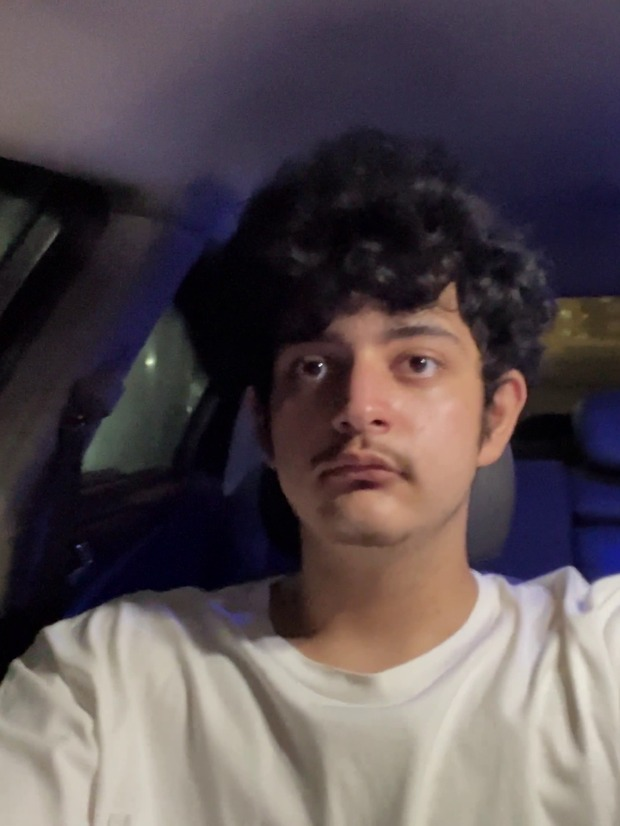
\includegraphics[width=\linewidth]{Figures/pilot/grid_1.jpg}\caption{C1: night, low on the dash}\end{subfigure}\hfill
  \begin{subfigure}[t]{0.24\linewidth}\centering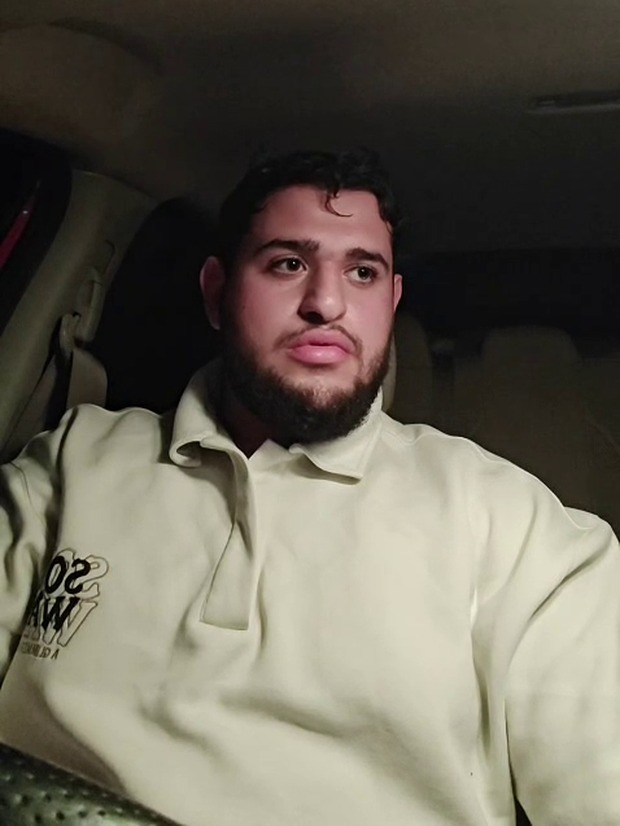
\includegraphics[width=\linewidth]{Figures/pilot/grid_2.jpg}\caption{C2: night, on the dash}\end{subfigure}\hfill
  \begin{subfigure}[t]{0.24\linewidth}\centering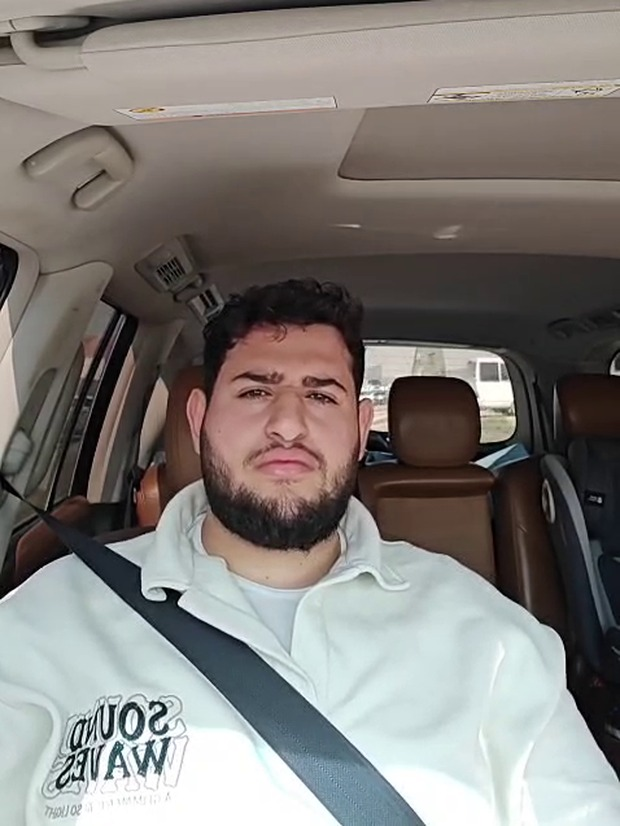
\includegraphics[width=\linewidth]{Figures/pilot/grid_3.jpg}\caption{C3: day, on the dash}\end{subfigure}\hfill
  \begin{subfigure}[t]{0.24\linewidth}\centering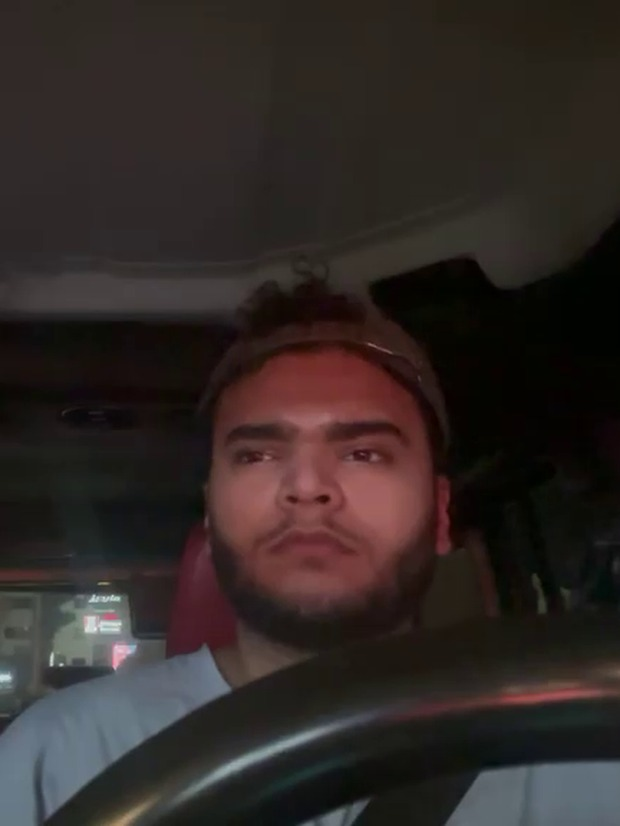
\includegraphics[width=\linewidth]{Figures/pilot/grid_4.jpg}\caption{C4: night, below the wheel}\end{subfigure}
  \caption{One frame from each pilot session, turned upright where needed}
  \label{fig:ch5-pilot}
\end{figure}

Figure \ref{fig:ch5-lessons} and Table \ref{tab:ch5-lessons} summarise what the sessions taught us, with each lesson visible in its frame. Figure \ref{fig:ch5-night} follows one drive in C4, where within 25\,s the same face turns green, red, evenly lit and dark. An \gls{rgb} camera captures all of this variation, which is why training uses hue and brightness augmentation (Table \ref{tab:ch4-14}) and why an \gls{ir} camera remains the first Future item.

\begin{figure}[htbp]
  \centering
  \begin{subfigure}[t]{0.24\linewidth}\centering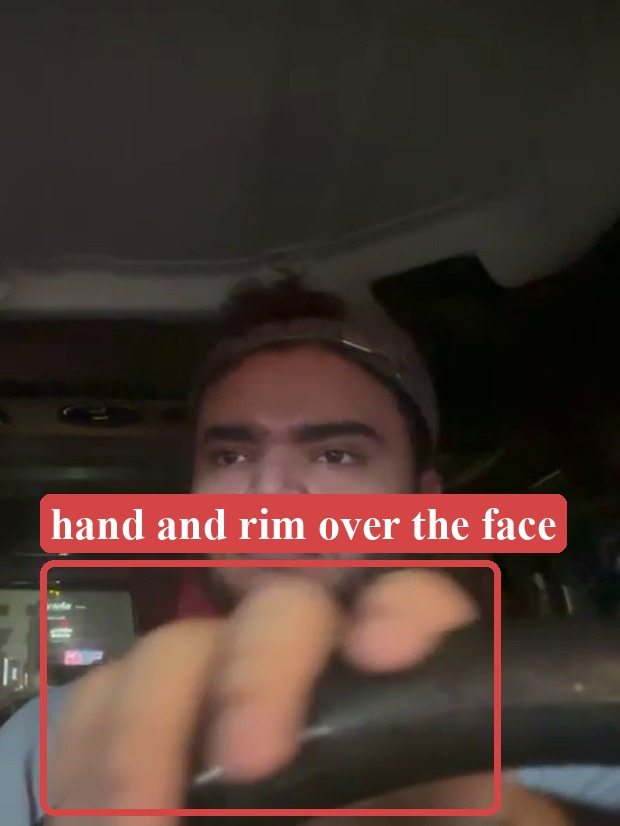
\includegraphics[width=\linewidth]{Figures/pilot/lesson_a.jpg}\caption{Below the wheel, the hand and rim hide the face}\end{subfigure}\hfill
  \begin{subfigure}[t]{0.24\linewidth}\centering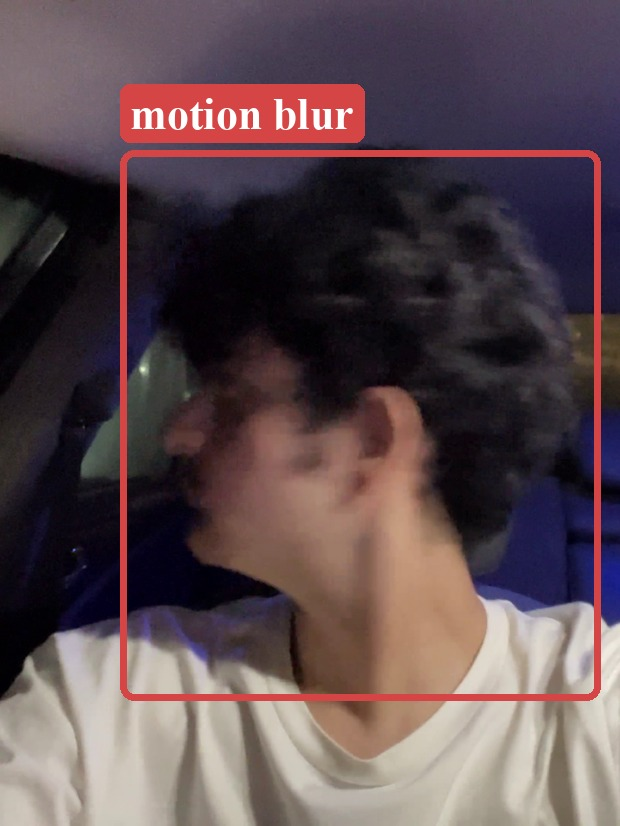
\includegraphics[width=\linewidth]{Figures/pilot/lesson_b.jpg}\caption{A fast head turn blurs at 14 \glsentryshort{fps}}\end{subfigure}\hfill
  \begin{subfigure}[t]{0.24\linewidth}\centering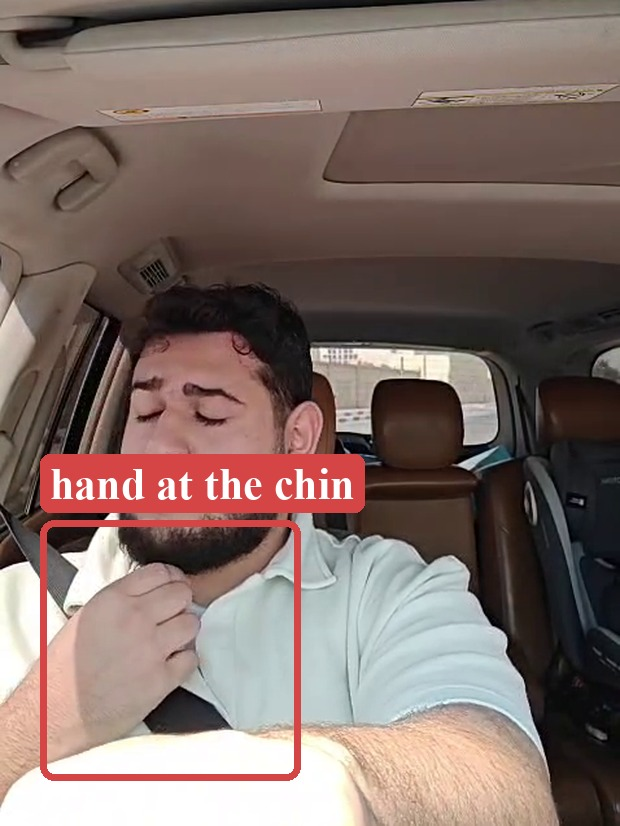
\includegraphics[width=\linewidth]{Figures/pilot/lesson_c.jpg}\caption{A hand at the chin with the eyes shut}\end{subfigure}\hfill
  \begin{subfigure}[t]{0.24\linewidth}\centering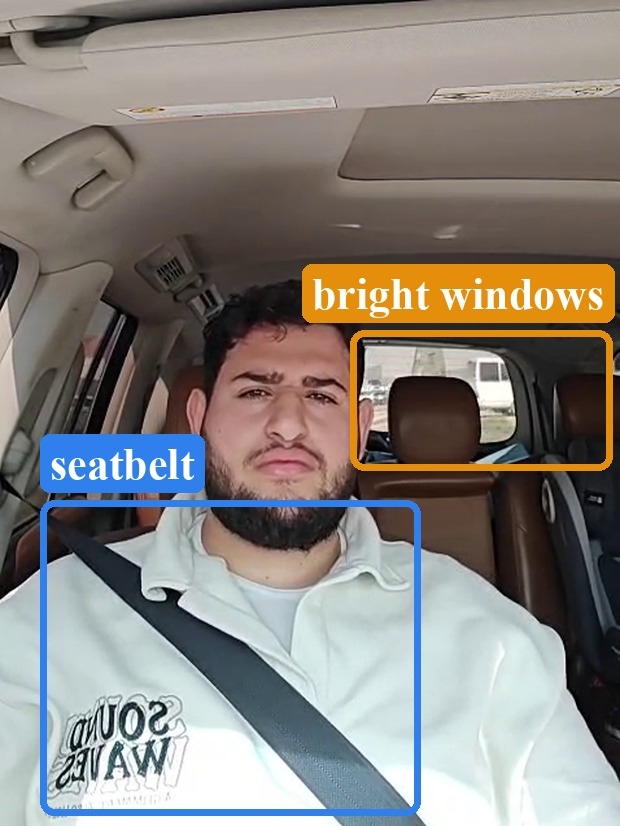
\includegraphics[width=\linewidth]{Figures/pilot/lesson_d.jpg}\caption{Bright windows and a seatbelt in daylight}\end{subfigure}
  \caption{What the pilot sessions showed, with the problem marked in each frame (Table \ref{tab:ch5-lessons})}
  \label{fig:ch5-lessons}
\end{figure}

\begin{table}[htbp]
\centering
\caption{What the pilot sessions taught us}
\label{tab:ch5-lessons}
\footnotesize
\setlength{\tabcolsep}{3pt}
\renewcommand{\arraystretch}{1.15}
\begin{tabular}{|p{0.060\linewidth}|p{0.420\linewidth}|p{0.450\linewidth}|}
\hline
\textbf{Frame} & \textbf{What we saw} & \textbf{What we do} \\
\hline
(a) & Below the wheel, the rim and the hand cross the face & Keep the dash-top mount above the column (Section 4.3.3) \\
\hline
(b) & A fast head turn is blurred at 14 \gls{fps} & Record at 30 \gls{fps} with the C922, and keep the 3\,s rule so one blurred frame never reads as a blocked camera \\
\hline
(c) & A hand at the chin and neck, with the eyes shut and the head turned & Keep the chin row in the hard-negative list (Table \ref{tab:ch5-04}), and test the eye rule with the head turned and down (T-20) \\
\hline
(d) & Bright rear windows behind the driver in daylight, and a seatbelt across the chest & Set the camera exposure for the face, not the whole frame, and treat the seatbelt as part of a normal pose \\
\hline
\end{tabular}
\end{table}

\begin{figure}[htbp]
  \centering
  \begin{subfigure}[t]{0.24\linewidth}\centering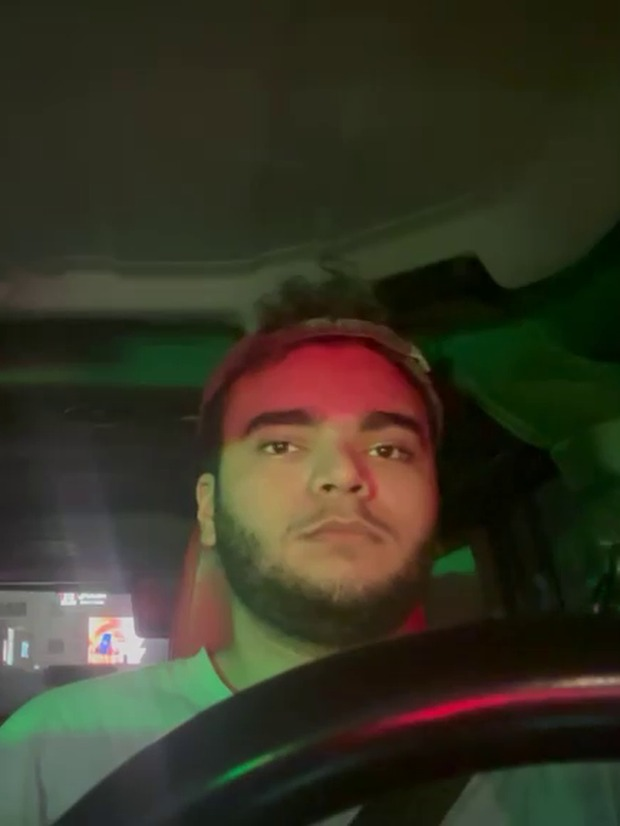
\includegraphics[width=\linewidth]{Figures/pilot/night_1.jpg}\caption{3.0\,s: green light}\end{subfigure}\hfill
  \begin{subfigure}[t]{0.24\linewidth}\centering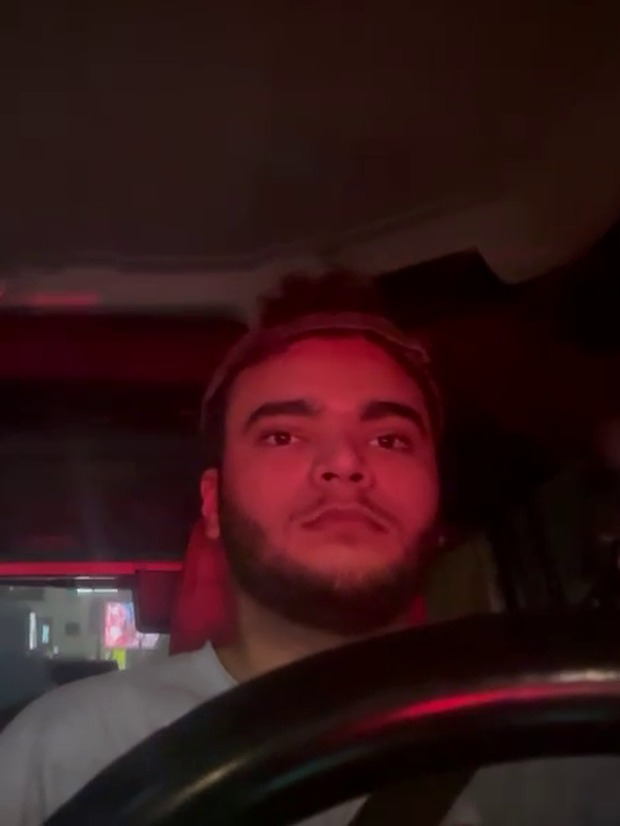
\includegraphics[width=\linewidth]{Figures/pilot/night_2.jpg}\caption{4.2\,s: red light}\end{subfigure}\hfill
  \begin{subfigure}[t]{0.24\linewidth}\centering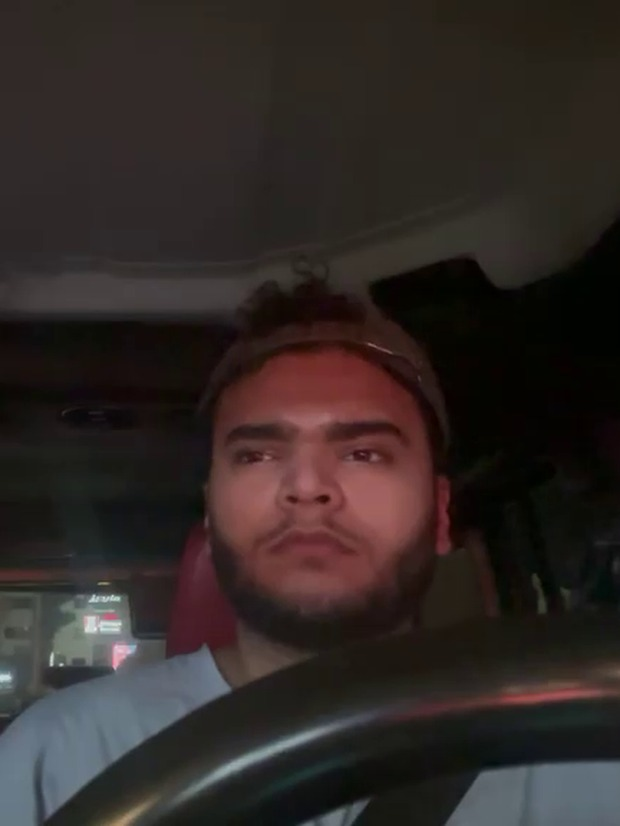
\includegraphics[width=\linewidth]{Figures/pilot/night_3.jpg}\caption{8.9\,s: even light}\end{subfigure}\hfill
  \begin{subfigure}[t]{0.24\linewidth}\centering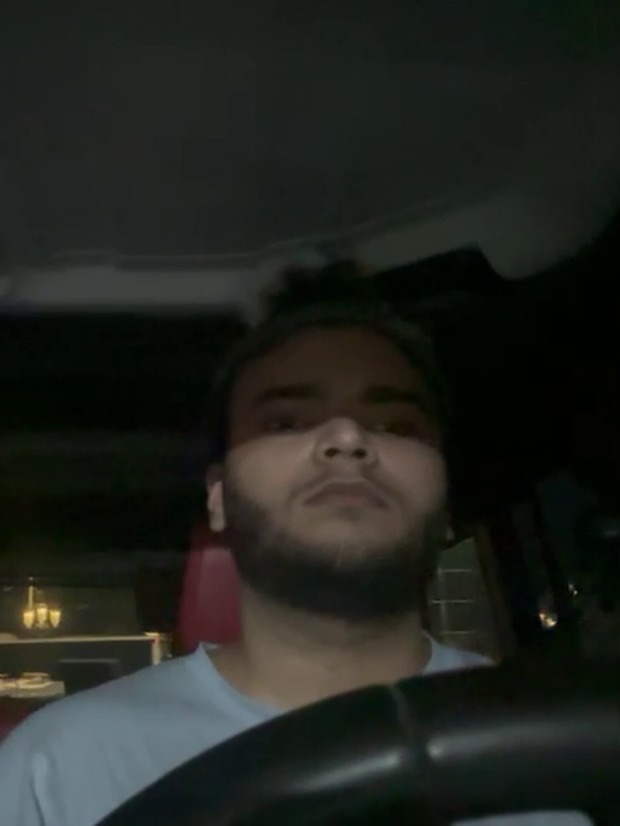
\includegraphics[width=\linewidth]{Figures/pilot/night_4.jpg}\caption{24.3\,s: almost dark}\end{subfigure}
  \caption{One night drive (C4): street light changes the colour and brightness of the same face within 25\,s}
  \label{fig:ch5-night}
\end{figure}

\subsubsection{Subjects and data handling}

The subjects are the four authors, so no outside participants are recorded and each author has agreed to appear in the dataset and in this report. Only an anonymised ID (S01 to S04) appears in file names and labels, and the videos stay on an encrypted university drive with access limited to the team and the supervisor. Since we plan to release the dataset publicly, each author may still withdraw their clips before the release.

\subsubsection{Neutral baseline clips}

Before each session, the subject sits normally for 20\,s. These clips serve two purposes: benchmarking the new-driver calibration of Section \ref{sec:calib} on people the model has not seen, and measuring each subject's open-eye \gls{ear} for the eye module.

\subsection{Labelling}
\subsubsection{Class definitions and annotation rules}

A positive must be visible for at least 0.5\,s, with the box covering the region that defines the class. Look-alikes are deliberately labelled as negatives, and head orientation is never labelled, so mirror checks and looking-away segments always remain negatives. Table \ref{tab:ch5-02} gives the rules.

\begin{table}[htbp]
\centering
\caption{Class definitions and annotation rules}
\label{tab:ch5-02}
\footnotesize
\setlength{\tabcolsep}{3pt}
\renewcommand{\arraystretch}{1.15}
\begin{tabular}{|p{0.150\linewidth}|p{0.300\linewidth}|p{0.280\linewidth}|p{0.190\linewidth}|}
\hline
\textbf{Class} & \textbf{Positive definition} & \textbf{Look-alikes (negative)} & \textbf{Box rule} \\
\hline
Yawning & Mouth wide open with jaw dropped, at least 0.5\,s & Talking, singing, laughing & Mouth and chin \\
\hline
Hand-over-mouth & Palm or back of hand covering the mouth & Touching nose or chin, adjusting headscarf & Hand and mouth region \\
\hline
Drinking & Bottle or cup at the lips & Holding a cup below the chin, eating & Container and mouth \\
\hline
Phone use & Phone at the ear or held in view and looked at & Hand at the cheek, phone in a holder & Phone and hand \\
\hline
\end{tabular}
\end{table}

\subsubsection{Annotation tool and quality checks}

Labels are drawn in CVAT on frames sampled at 5 \gls{fps}, with interpolation between key frames to speed up long cues. For the first subject, two annotators label each video independently, measuring agreement as the share of boxes that match at an \gls{iou} of 0.5 or more and discussing disagreements to refine the rules in Table \ref{tab:ch5-02}. From then on, one annotator labels each video and the second checks a random 10\% of frames, relabelling any video where more than 5\% of the checked frames disagree.

\subsection{Subject-disjoint evaluation with four subjects}

With only four subjects, a fixed split would leave a single person in the test set, so we use leave-one-subject-out testing instead. The model is first fine-tuned on the 14 drivers of DMD, then on our data in four folds, where each fold holds out one subject for testing and one for validation and trains on the remaining two, so that
\begin{equation}
\mathcal{S}_\text{train} \cap \mathcal{S}_\text{val} = \mathcal{S}_\text{train} \cap \mathcal{S}_\text{test} = \mathcal{S}_\text{val} \cap \mathcal{S}_\text{test} = \varnothing \quad \text{in every fold.}
\end{equation}
Every session, baseline clip and hard-negative clip of a subject stays with that subject. Results are reported as the mean and spread over the four folds, ensuring every subject is tested exactly once by a model that never saw them. Figure \ref{fig:ch5-04} shows the folds.

\begin{figure}[htbp]
\centering
\begin{tikzpicture}[font=\footnotesize]
  \foreach \f/\te/\va in {1/1/2, 2/2/3, 3/3/4, 4/4/1} {
    \node[anchor=east] at (-0.2,-\f*0.8) {Fold \f};
    \foreach \s in {1,...,4} {
      \ifnum\s=\te \def\c{sbred}\def\l{Test}\else\ifnum\s=\va \def\c{sbgold}\def\l{Val}\else\def\c{sbblue}\def\l{Train}\fi\fi
      \node[draw=\c, line width=0.9pt, fill=\c!12, minimum width=20mm, minimum height=6mm] at (\s*2.3,-\f*0.8) {\l};
    }
  }
  \foreach \s in {1,...,4} \node[font=\footnotesize\bfseries] at (\s*2.3,0) {S0\s};
\end{tikzpicture}
\caption{Leave-one-subject-out folds: every subject is tested once by a model that never saw them}
\label{fig:ch5-04}
\end{figure}

\subsection{Hard-negative dataset}

After the first model is trained, we run it at a low confidence on the training and validation clips and collect the frames it wrongly flags. The same subjects then record a short session deliberately acting these look-alikes (Table \ref{tab:ch5-04}). Only negative frames are added, with each subject kept in their own split, and false alarms per hour are compared before and after, using the 40\% hard-mined ratio from Chapter 1.

\begin{table}[htbp]
\centering
\caption{Planned hard negatives}
\label{tab:ch5-04}
\footnotesize
\setlength{\tabcolsep}{3pt}
\renewcommand{\arraystretch}{1.15}
\begin{tabular}{|p{0.430\linewidth}|p{0.260\linewidth}|p{0.240\linewidth}|}
\hline
\textbf{Look-alike behaviour} & \textbf{Class it may fool} & \textbf{Frames added (target)} \\
\hline
Talking, singing, laughing & Yawning & About 800 \\
\hline
Rubbing nose or chin, adjusting headscarf or glasses & Hand-over-mouth & About 800 \\
\hline
Holding a cup below the chin, eating a snack & Drinking & About 600 \\
\hline
Hand resting on the cheek, touching the ear & Phone use & About 600 \\
\hline
Phone in a dashboard holder, not held & Phone use & About 400 \\
\hline
\end{tabular}
\end{table}

\section{How We Will Prove It Works}
\subsection{What will be verified: each specification matched to a test}

Every specification of Tables \ref{tab:req-features} and \ref{tab:desired-features} maps to at least one verification method: test (measured against a pass criterion), analysis (calculation or review of logs), inspection (checking the build or the code) or demonstration (showing the feature working with a user). Test T-$xx$ verifies specification FS-$xx$, and Table \ref{tab:ch5-07} lists the main feature tests.

\subsection{Test procedures}
\subsubsection{Model tests on the subject-disjoint test set}

The final model is tested leave-one-subject-out on our four subjects, as well as on the three held-out DMD drivers. We report per-class precision, recall, F1 and \gls{map} with a confusion matrix, computed per frame, while false alarms per hour are computed on the full pipeline output over the neutral and hard-negative clips, before and after hard-negative retraining. The test split is never used to tune cutoffs or $\tau$.

\subsubsection{Performance tests on the Raspberry Pi 5}

Each model variant runs on the Pi for 30 minutes on a recorded test clip in a room at about 30\,$^\circ$C, with the case closed and the cooler running. We log \gls{fps}, end-to-end latency (mean and 95th percentile), SoC temperature and any throttling flags reported by the firmware, alongside the accuracy of the same variant on the validation set. The variants are the baseline at 640 and 320 px on the CPU, the baseline on the Hailo \gls{npu}, and 20\% and 30\% pruned models on the \gls{npu}, each with \gls{ptq} and \gls{qat}.


\subsubsection{Feature tests}

Each feature has a simple, repeatable test (Table \ref{tab:ch5-07}). Eye closure is tested on the demonstration rig of Section \ref{sec:demo}, including closures with the head down, since these were confused on the DMD footage. All feature tests run on the same rig, always with subjects whose clips were not used for training.

{\footnotesize
\setlength{\tabcolsep}{3pt}
\renewcommand{\arraystretch}{1.12}
\begin{longtable}{|p{0.075\linewidth}|p{0.210\linewidth}|p{0.360\linewidth}|p{0.290\linewidth}|}
\caption{Feature tests}
\label{tab:ch5-07}\\
\hline
\textbf{Test ID} & \textbf{Feature} & \textbf{Procedure} & \textbf{Pass criterion} \\
\hline
\endfirsthead
\hline
\textbf{Test ID} & \textbf{Feature} & \textbf{Procedure} & \textbf{Pass criterion} \\
\hline
\endhead
\hline
\endfoot
T-04 & \gls{ema} filter & Replay one clip at 10, 15 and 30 \gls{fps} & Confirmation times agree within one frame \\ \hline
T-05 & Light and voice alert & Film the bar at 240 \gls{fps} and listen to the message & $\le$ 3 flashes/s and the message plays after every confirmed event \\ \hline
T-06 & Cool-down & Two same-class cues 10\,s apart & Second cue not alerted, both logged \\ \hline
T-07 & Mirror checks & 20 scripted mirror checks & No alert \\ \hline
T-15 & Escalation & Hold a cue for 15\,s & Tier 2 at 5\,s, Tier 3 at 10\,s ($\pm$0.2\,s) \\ \hline
T-16 & Explained messages & Trigger each class & Message names class and count or duration \\ \hline
T-17 & Camera-blind check & Cover the lens or shine a torch, 10 trials each & Announcement within 3--3.5\,s in all trials \\ \hline
T-18 & Crop tracking & Same clips, fixed vs tracked & Tracked recall $\ge$ fixed, no extra false alarms \\ \hline
T-19 & Calibration & Test subjects' baselines & False alarms/h not higher than defaults \\ \hline
T-20 & Eye closure & Acted closures of 1, 1.5 and 2\,s, and 2 and 4\,s with the head down & Alert at 1.5\,s and 2\,s, none at 1\,s, and with the head down none at 2\,s and alert at 3\,s \\ \hline
T-24 & Display & Five users perform setup and read status & All complete setup unaided and read the status in under 2\,s \\ \hline
T-26 & Rest-stop suggestion & Simulate high alert rate at a known location & Nearest \gls{poi} named within 5\,s \\ \hline
T-21 & Power-cut logging & A smart relay cuts power 50 times during writes & Integrity check passes, no committed event lost \\ \hline
T-22 & Secure upload & Upload to a server with a bad certificate, and drop Wi-Fi during an upload & Upload refused, no event lost or duplicated, no readable traffic \\ \hline
-- & Endurance & Two-hour continuous run & No memory leak, throttling or missed frames \\ \hline
\end{longtable}
}


\subsection{Expected results and pass/fail criteria}

Required specifications are must-pass, so a failure is fixed before any Desired feature is added. Desired specifications are aims, and a miss is reported with its cause rather than blocking the project. Table \ref{tab:ch5-08} gives the target and minimum acceptable value for the key specifications.

\begin{table}[htbp]
\centering
\caption{Expected results and pass/fail criteria}
\label{tab:ch5-08}
\footnotesize
\setlength{\tabcolsep}{3pt}
\renewcommand{\arraystretch}{1.15}
\begin{tabular}{|p{0.100\linewidth}|p{0.250\linewidth}|p{0.250\linewidth}|p{0.120\linewidth}|p{0.180\linewidth}|}
\hline
\textbf{Spec} & \textbf{Target} & \textbf{Minimum acceptable} & \textbf{Type} & \textbf{Result (SDP~2)} \\
\hline
FS-01 & 30 \gls{fps}, $\le$ 60 ms & 25 \gls{fps}, $\le$ 100 ms & Must pass & \\
\hline
FS-03 & Recall $\ge$ 0.95 & Recall $\ge$ 0.90 & Must pass & \\
\hline
FS-04 & Agreement within 1 frame & Within 2 frames & Must pass & \\
\hline
FS-05 & $\le$ 3 flashes/s & $\le$ 3 flashes/s & Must pass & \\
\hline
FS-06 & No repeat in 30\,s & No repeat in 30\,s & Must pass & \\
\hline
System & $\le$ 3 false alarms/h & $<$ 10 false alarms/h & Must pass & \\
\hline
FS-11 & $\ge$ 40 \gls{fps} after compression & Recall drop $\le$ 2 points & Aim & \\
\hline
FS-17 & Detected in 3\,s & Detected in 4\,s & Aim & \\
\hline
FS-19 & 30\% fewer false alarms & Not more than default & Aim & \\
\hline
FS-20 & Alert at 1.5\,s & Alert by 2\,s & Aim & \\
\hline
FS-21 & 50/50 power cuts clean & 50/50 power cuts clean & Aim & \\
\hline
\end{tabular}
\end{table}

\section{Project Plan: Parts, Budget, Timeline and Risks}
\subsection{Hardware parts list}

Table \ref{tab:ch5-09} lists every item in our approved purchase request, all sourced from Amazon.ae for fast delivery in the \gls{uae}, with each supplier entry linking to the product page. The \gls{mosfet} and resistors for the light-bar driver come from the department lab stock at no cost. The AI HAT+ moved from optional to Required once our compute estimate showed that the CPU alone cannot reach the target \gls{fps}, and the PXN wheel serves both the demonstration rig and the prototype of the Future steering-wheel alert.

\begin{table}[htbp]
\centering
\caption{Hardware parts list and estimated budget}
\label{tab:ch5-09}
\footnotesize
\setlength{\tabcolsep}{3pt}
\renewcommand{\arraystretch}{1.15}
\begin{tabular}{|p{0.040\linewidth}|p{0.300\linewidth}|p{0.120\linewidth}|p{0.050\linewidth}|p{0.120\linewidth}|p{0.100\linewidth}|p{0.150\linewidth}|}
\hline
\textbf{\#} & \textbf{Item} & \textbf{Supplier} & \textbf{Qty} & \textbf{Unit (\gls{aed})} & \textbf{Total} & \textbf{Status} \\
\hline
1 & Raspberry Pi 5 (8 GB) & \href{https://www.amazon.ae/dp/B0CK2FCG1K}{\textcolor{own1}{Amazon.ae}} & 1 & 845 & 845 & Required \\ \hline
2 & Raspberry Pi AI HAT+ & \href{https://www.amazon.ae/dp/B0DKTTDW79}{\textcolor{own1}{Amazon.ae}} & 1 & 391 & 391 & Required \\ \hline
3 & Logitech C922 webcam & \href{https://www.amazon.ae/dp/B01MTTMPKT}{\textcolor{own1}{Amazon.ae}} & 1 & 255 & 255 & Required \\ \hline
4 & Creative Pebble V3 speakers & \href{https://www.amazon.ae/dp/B08F5BQZL8}{\textcolor{own1}{Amazon.ae}} & 1 & 177 & 177 & Required \\ \hline
5 & 27 W \gls{usb}-C power supply & \href{https://www.amazon.ae/dp/B0D4DM1D21}{\textcolor{own1}{Amazon.ae}} & 1 & 112 & 112 & Required \\ \hline
6 & Raspberry Pi 5 Active Cooler & \href{https://www.amazon.ae/dp/B0CW164TCW}{\textcolor{own1}{Amazon.ae}} & 1 & 64 & 64 & Required \\ \hline
7 & SanDisk Extreme Pro 128 GB & \href{https://www.amazon.ae/dp/B0DCW7MST8}{\textcolor{own1}{Amazon.ae}} & 1 & 136 & 136 & Required \\ \hline
8 & Metal case & \href{https://www.amazon.ae/dp/B0DGTMXWHT}{\textcolor{own1}{Amazon.ae}} & 1 & 86 & 86 & Required \\ \hline
9 & UGREEN micro-\gls{usb} cable & \href{https://www.amazon.ae/dp/B01NCJE1RE}{\textcolor{own1}{Amazon.ae}} & 1 & 22 & 22 & Desired \\ \hline
10 & Hosyond 7-inch touch display & \href{https://www.amazon.ae/dp/B09XKC53NH}{\textcolor{own1}{Amazon.ae}} & 1 & 245 & 245 & Desired \\ \hline
11 & KABCON tablet holder & \href{https://www.amazon.ae/dp/B092C6LZGS}{\textcolor{own1}{Amazon.ae}} & 1 & 44 & 44 & Desired \\ \hline
12 & UGREEN \gls{usb} 3.0 hub & \href{https://www.amazon.ae/dp/B0CD1BHXPZ}{\textcolor{own1}{Amazon.ae}} & 1 & 28 & 28 & Required \\ \hline
13 & \gls{rgb} light bar & \href{https://www.amazon.ae/dp/B0F93X6L1C}{\textcolor{own1}{Amazon.ae}} & 1 & 70 & 70 & Required \\ \hline
14 & PXN steering wheel & \href{https://www.amazon.ae/dp/B08BLMP4ZR}{\textcolor{own1}{Amazon.ae}} & 1 & 250 & 250 & Future (prototype) \\ \hline
-- & Logic-level \gls{mosfet}, 220\,$\Omega$ and 10\,k$\Omega$ resistors, jumpers & Lab stock & -- & 0 & 0 & Required \\ \hline
\multicolumn{5}{|r|}{\textbf{Grand total}} & \textbf{2725} & \\
\hline
\end{tabular}
\end{table}


\subsection{Project budget}

The department funds the approved purchase request against a cap of 5000 \gls{aed}. With a 15\% contingency for spares, a car power adapter and cables, the total comes to about 3134 \gls{aed} (Table \ref{tab:ch5-10}).

\begin{table}[htbp]
\centering
\caption{Project budget (\glsentryshort{aed})}
\label{tab:ch5-10}
\footnotesize
\setlength{\tabcolsep}{3pt}
\renewcommand{\arraystretch}{1.15}
\begin{tabular}{|p{0.330\linewidth}|p{0.140\linewidth}|p{0.140\linewidth}|p{0.140\linewidth}|p{0.140\linewidth}|}
\hline
\textbf{Category} & \textbf{Required} & \textbf{Desired} & \textbf{Future} & \textbf{Total} \\
\hline
Hardware & 2164 & 311 & 250 & 2725 \\
\hline
Software and services & 0 & 0 & 0 & 0 \\
\hline
Contingency (15\%) & 325 & 47 & 37 & 409 \\
\hline
\textbf{Total} & \textbf{2489} & \textbf{358} & \textbf{287} & \textbf{3134} \\
\hline
\end{tabular}
\end{table}

\subsection{Timeline and resource plan for SDP2}
\subsubsection{Milestones and Gantt chart}

Required features come first and data collection starts early, as recording, labelling and the hard-negative round form the bottleneck. The Required build is frozen by week 8, after which the Desired features follow in priority order with a buffer for the Eid al-Fitr break, testing runs in weeks 13 to 15, and the final two weeks are reserved for the report, poster and presentation (Figure \ref{fig:ch5-07}).

\begin{figure}[htbp]
\centering
\resizebox{\linewidth}{!}{%
\begin{ganttchart}[
  hgrid, vgrid={*{6}{draw=none},dotted}, x unit=0.11cm, y unit chart=0.62cm,
  time slot format=isodate, title height=1, bar height=0.5,
  bar/.append style={fill=sbblue!35, draw=sbblue}, milestone/.append style={fill=sbred, draw=sbred},
  bar label font=\small, milestone label font=\small\itshape, title label font=\small]{2027-01-18}{2027-05-23}
  \gantttitlecalendar{month=name} \\
  \ganttbar{Parts, bench assembly and wiring}{2027-01-18}{2027-02-07} \\
  \ganttbar{Recording and labelling}{2027-01-25}{2027-03-07} \\
  \ganttbar{Required pipeline on the Pi}{2027-02-01}{2027-03-07} \\
  \ganttmilestone{Required features frozen}{2027-03-07} \\
  \ganttbar[bar/.append style={fill=gray!35, draw=gray}]{Eid al-Fitr break (approx.)}{2027-03-08}{2027-03-13} \\
  \ganttbar[bar/.append style={fill=sbgreen!35, draw=sbgreen}]{Desired features}{2027-03-14}{2027-04-18} \\
  \ganttbar[bar/.append style={fill=sbgreen!35, draw=sbgreen}]{Hard-negative round}{2027-03-22}{2027-04-04} \\
  \ganttbar[bar/.append style={fill=sbgold!35, draw=sbgold}]{Testing}{2027-04-12}{2027-05-02} \\
  \ganttbar[bar/.append style={fill=sbgold!35, draw=sbgold}]{Report, poster and presentation}{2027-05-03}{2027-05-16} \\
  \ganttmilestone{SDP~2 demonstration}{2027-05-19}
\end{ganttchart}}
\caption{Gantt chart for SDP~2}
\label{fig:ch5-07}
\end{figure}


\subsubsection{Task assignment for each team member}

Each task has one owner and one support member who can take over (Table \ref{tab:ch5-12}).

\begin{table}[htbp]
\centering
\caption{Task assignment}
\label{tab:ch5-12}
\footnotesize
\setlength{\tabcolsep}{3pt}
\renewcommand{\arraystretch}{1.15}
\begin{tabular}{|p{0.360\linewidth}|p{0.190\linewidth}|p{0.190\linewidth}|p{0.170\linewidth}|}
\hline
\textbf{Task} & \textbf{Owner} & \textbf{Support} & \textbf{Due (approx.)} \\
\hline
Dataset collection and labelling & Oumar & Mohamed & 7 Mar 2027 \\
\hline
Training, pruning, hard negatives & Oumar & Abdullah & 4 Apr 2027 \\
\hline
Bench assembly, wiring, power & Abdullah & Faris & 7 Feb 2027 \\
\hline
Hailo compile and on-device pipeline & Abdullah & Oumar & 21 Feb 2027 \\
\hline
\gls{ema}, decision logic, alerts, logging & Abdullah & Mohamed & 7 Mar 2027 \\
\hline
Upload \gls{api}, database, dashboard & Faris & Oumar & 11 Apr 2027 \\
\hline
Display \gls{ui}, calibration screens, voice messages & Mohamed & Faris & 3 Apr 2027 \\
\hline
Eye module and crop tracking & Oumar & Abdullah & 18 Apr 2027 \\
\hline
Testing and user trials & Mohamed & All & 2 May 2027 \\
\hline
Final report and poster & All & All & 16 May 2027 \\
\hline
\end{tabular}
\end{table}

\subsection{Risks and backup plans}

Table \ref{tab:ch5-13} lists each risk with its likelihood, impact and mitigation. The largest risks are delays in data collection and poor generalisation from only four subjects, which we address by starting early, pre-training on public data and calibrating per driver.

\begin{table}[htbp]
\centering
\caption{Risks and backup plans}
\label{tab:ch5-13}
\footnotesize
\setlength{\tabcolsep}{3pt}
\renewcommand{\arraystretch}{1.15}
\begin{tabular}{|p{0.050\linewidth}|p{0.240\linewidth}|p{0.110\linewidth}|p{0.100\linewidth}|p{0.420\linewidth}|}
\hline
\textbf{ID} & \textbf{Risk} & \textbf{Likelihood} & \textbf{Impact} & \textbf{Mitigation} \\
\hline
R1 & Data-collection delays & Likely & High & Four pilot sessions are already recorded (Section \ref{sec:pilot}). Book slots in week 1, record two sessions per day and fall back on DMD and YawDD for missing classes \\
\hline
R2 & Poor generalisation to new subjects & Likely & High & Only four subjects: pre-train on 14 DMD drivers, leave-one-subject-out testing, per-driver calibration, hard negatives \\
\hline
R3 & Pi too slow or too hot & Possible & Moderate & AI HAT+, 320 px CPU fallback, active cooler, vented case \\
\hline
R4 & Too few hard negatives & Possible & Low & Script look-alikes in advance and mine false positives from public sets \\
\hline
R5 & Demonstration room differs from the recorded cars & Possible & Moderate & Per-driver calibration at the start of each demonstration, brightness and hue augmentation, and the blind check \\
\hline
R6 & Supply delays & Possible & Moderate & Order in week 1, with local alternatives for every part \\
\hline
R7 & Hailo compile issues & Unlikely & Low & Use Hailo Model Zoo configs for \gls{yolo}11n, with a CPU fallback \\
\hline
R8 & Map and \gls{poi} service access & Likely & Low & Overpass \gls{api} needs no key but live queries timed out in our tests, so a saved list of 363 places answers within the limit \\
\hline
R9 & Eye alarm false alerts & Likely & High & Record real closures at full frame rate, retune on the C922, and keep the alarm out of the frozen build until it meets the target \\
\hline
\end{tabular}
\end{table}
